\documentclass[11pt]{article}

% ==== Paquetes ====
\usepackage[utf8]{inputenc}
\usepackage[spanish]{babel}
\usepackage{listingsutf8}
\usepackage{amsmath, amssymb, amsfonts, siunitx}
\usepackage{graphicx}
\usepackage{float}
\usepackage{minted}   % Para código con sintaxis coloreada
\usepackage{xcolor}
\usepackage{hyperref}
\usepackage{caption}
\usepackage{subcaption}
\usepackage{geometry}
\usepackage{listings}
\usepackage{tikz}

\lstdefinestyle{mypython}{
    language=Python,
    backgroundcolor=\color{black!5},
    commentstyle=\color{green!50!black},
    keywordstyle=\color{blue},
    numberstyle=\tiny\color{gray},
    stringstyle=\color{red!60!black},
    basicstyle=\ttfamily\small,
    breaklines=true,
    numbers=left,
    numbersep=5pt,
    frame=single,
    rulecolor=\color{black!30},
    showstringspaces=false,
    tabsize=4,
    upquote=true,
    basicstyle=\fontencoding{T1}\selectfont,
    inputencoding=utf8/latin1
}

\geometry{margin=2.5cm}

% ==== Datos de la tarea ====
\title{IEE3584 - Comunicaciones inalámbricas \\
Tarea 5}
\author{Nicolás Seguel}
\date{Septiembre 2025}

\begin{document}
\maketitle

\section*{Problema 15:}

\subsection*{a) Grafique la respuesta de impulso y respuesta de frecuencia del canal.}

\begin{figure}[H]
    \begin{subfigure}[b]{0.45\textwidth}
        \centering
        \includegraphics[width=\textwidth]{H_time_domain.png}
        \caption{Respuesta al impulso $h(t)$}
        \label{fig:H_time_domain}
    \end{subfigure}
    \hfill
    \begin{subfigure}[b]{0.45\textwidth}
        \centering
        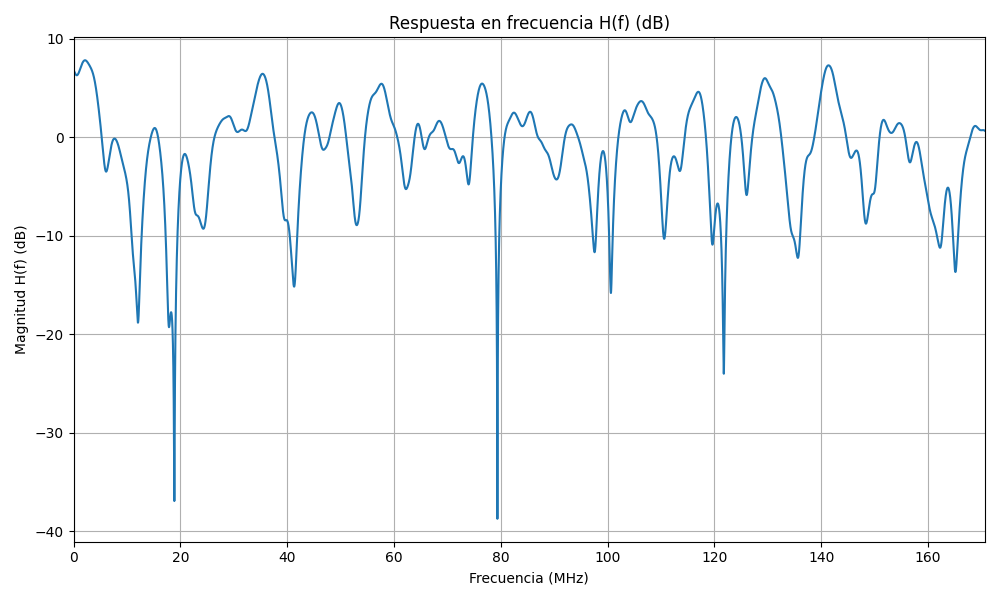
\includegraphics[width=\textwidth]{H_freq_domain.png}
        \caption{Respuesta en frecuencia $H(f)$}
        \label{fig:H_freq_domain}
    \end{subfigure}
    \caption{Respuesta del canal en tiempo y frecuencia}
    \label{fig:H_channel}
\end{figure}

A partir de los datos en los archivos de texto, se obtiene la respuesta al impulso del canal $h(t)$ directamente. Luego, se calcula su transformada de Fourier para obtener la respuesta en frecuencia $H(f)$.

\subsection*{b) Calcule el retardo excesivo medio de este canal.}

El retardo excesivo medio se calcula como:

\[
\tau_{mean} = \frac{\sum_i \tau_i |h(\tau_i)|^2}{\sum_i |h(\tau_i)|^2}
\]

Donde $\tau_i$ son los tiempos de retardo y $h(\tau_i)$ es la respuesta al impulso en esos tiempos. Esta suma pondera los retardos por la potencia recibida en cada uno. El resultado numérico es:

\[
\tau_{mean} = 70.696 \, ns
\]

\subsection*{c) Calcule el valor RMS de la dispersión del canal.}

El valor RMS de la dispersión del canal se calcula como:

\[
\tau_{rms} = \sqrt{\frac{\sum_i (\tau_i - \tau_{mean})^2 |h(\tau_i)|^2}{\sum_i |h(\tau_i)|^2}}
\]

El resultado numérico es:

\[
\tau_{rms} = 68.762 \, ns
\]

\subsection*{d) Calcule el ancho de banda de coherencia del canal.}

El ancho de banda de coherencia $\omega_c$ se puede estimar usando la regla empírica:

\[
\omega_c \approx \frac{1}{5 \tau_{rms}} \quad \text{o} \quad \omega_c \approx \frac{1}{50 \tau_{rms}}
\]

Siendo el valor más estricto el de $1/(50 \tau_{rms})$ y el valor más laxo es $1/(50 \tau_{rms})$. Los resultados numéricos son:

\[
\omega_{c} = \left[ 0.291 \, MHz , 2.91 \, MHz \right]
\]

\subsection*{e) ¿Qué tipo de desvanecimiento enfrenta la transmisión digital a través de este canal, selectivo o plano en frecuencia?}

Considerando que se tiene una modulación 64-QAM con una tasa de datos de 254 Mbps, la tasa de símbolo es:

\[
R_s = \frac{254 \, Mbps}{6 \, bits/simbolo} \approx 42.33 \, MHz
\]

Comparando la tasa de símbolo con los anchos de banda de coherencia calculados:

\[
\omega_{c} = \left[ 0.291 \, MHz , 2.91 \, MHz \right] < R_s = 42.33 \, MHz
\]

Dado que la tasa de símbolo es mucho mayor que el ancho de banda de coherencia, el canal es \textbf{selectivo en frecuencia}.

\section*{Problema 16:}

Se tiene un sistema de comunicación inalámbrica dentro de un taller pequeño de $100 \, m^2$. Asumiendo que la habitación es cuadrada, el tiempo de retardo del primer eco se calcula como:

\[
\tau_0 = \frac{\SI{10}{m}}{c} \approx 33.33 \, ns
\]

Asumiendo un ambiente con respuesta al impulso exponencial, se puede asumir que el valor RMS de la dispersión del canal es aproximadamente igual al retardo del primer eco, ya que la mayoría de la energía se concentra en los primeros ecos y la dispersión es baja en un espacio pequeño y cerrado. Por lo tanto:

\[
\tau_{rms} \approx \tau_0
\]

El ancho de banda de coherencia se estima como:

\[
\omega_c = \left[ \frac{1}{5 \tau_{rms}}, \frac{1}{50 \tau_{rms}} \right] = \left[ 6 \, MHz , 600 \, kHz \right]
\]

Considerando que la correlación para el criterio estricto es de $0.9$ y para el laxo es de $0.5$, y que se busca una cobertura del $99.9\%$, el criterio laxo queda descartado por el bajo nivel de correlación. Por lo tanto, se utiliza el criterio estricto para determinar el ancho de banda de coherencia y se concluye que el canal es \textbf{selectivo en frecuencia} para un ancho de banda de transmisión de $4MHz$.

Asumiendo que se tiene un canal selectivo en frecuencia, no es posible calcular el presupuesto de enlace para las condiciones dadas, ya que el canal introduce distorsión intersimbólica (ISI) que no puede ser compensada simplemente con un margen de desvanecimiento. Para mitigar el ISI, se necesitarían técnicas adicionales como ecualización o modulación adaptativa.

\section*{Problema 17:}

\subsection*{a) Envolvente compleja de la respuesta al impulso}

La señal transmitida es
\[
p(t) = 2 \cos(2\pi f_c t)\, \mathrm{rect}\!\left(\frac{t - T_p/2}{T_p}\right)
      = \Re\left\{ 2\,\mathrm{rect}\!\left(\frac{t - T_p/2}{T_p}\right) e^{j2\pi f_c t} \right\}.
\]

De esta forma, la envolvente compleja del pulso es
\[
\tilde p(t) = 2\,\mathrm{rect}\!\left(\frac{t - T_p/2}{T_p}\right).
\]

La señal recibida, sin ruido, es
\[
r(t) = \sum_{n=1}^{L_c} h_n\,p(t-\tau_n).
\]

Usando la representación en banda base compleja se obtiene
\[
\tilde r(t) = \sum_{n=1}^{L_c} h_n\,\tilde p(t-\tau_n)\,e^{-j2\pi f_c \tau_n}.
\]

Por comparación con $\tilde r(t) = (\tilde h * \tilde p)(t)$, la envolvente compleja de la respuesta al impulso del canal resulta ser
\[
\tilde h(t) = \sum_{n=1}^{L_c} h_n \, e^{-j2\pi f_c \tau_n}\,\delta(t-\tau_n).
\]


\subsection*{b) Interpretación del perfil de retardos}

A partir de la Figura 2 se tienen los siguientes valores característicos del canal: 
\[
\bar\tau = 45.05\ \text{ns}, \qquad 
\tau_{\rm rms} = 46.40\ \text{ns}, \qquad 
\tau_{\max} \approx 84\ \text{ns}.
\]

El análisis de estos parámetros permite extraer información importante sobre el entorno de propagación. En primer lugar, el hecho de que el pulso de mayor intensidad corresponda al primero indica que la trayectoria directa es dominante, por lo que es probable que exista línea de visión entre transmisor y receptor. Aun así, se observan contribuciones significativas en retardos posteriores, lo que implica la presencia de múltiples trayectorias.

El valor de $\tau_{\rm rms} = 46.40$ ns revela que el canal presenta una dispersión temporal apreciable. Esta dispersión genera que distintas componentes de la señal lleguen desfasadas en el tiempo, lo que repercute en la correlación en frecuencia y, por ende, en el ancho de banda de coherencia del canal. Por lo que es probable que el canal sea selectivo en frecuencia para señales con anchos de banda moderados a altos.

\subsection*{c) Condición para evitar ISI y tasa máxima}

Para que la interferencia intersímbolo (ISI) sea despreciable, la duración de símbolo $T_s$ debe ser mucho mayor que la dispersión temporal del canal. En términos de la tasa de símbolos $R_s$ se requiere
\[
T_s = \frac{1}{R_s} \gg \tau_{\rm rms}
\quad \Longrightarrow \quad
R_s \ll \frac{1}{\tau_{\rm rms}}.
\]

Como la tasa de símbolos es proporcional al ancho de banda $W$, se obtiene la condición
\[
W \ll \frac{1}{\tau_{\rm rms}}.
\]

Con $\tau_{\rm rms} = 46.40\ \text{ns}$, se tiene
\[
\frac{1}{\tau_{\rm rms}} \approx 21.6\ \text{MHz}.
\]
Si aplicamos una regla práctica más estricta, por ejemplo $W \leq 1/(5\tau_{\rm rms})$, resulta
\[
W \lesssim 4.3\ \text{MHz}.
\]

Por lo tanto, la tasa máxima de transmisión con ISI despreciable se encuentra del orden de unos pocos Mbps.


\section*{Anexo: Código Python utilizado}

\lstinputlisting[style=mypython, caption={Código Python para el problema 15}, label={lst:codigo_python}]{pregunta15.py}

\end{document}
